\chapter{COORDINATE SYSTEMS}
A co-ordinate system is a mathematical tool to describe the position of an object. It  is used extensively in describing a physical problem or a situation . The information about problem of interest is depicted in 'co-ordinate', it is the set of two or more numbers that specifies the position of a point, line, or other geometric figure in relation to some reference system.\newline There are mainly four kinds of coordinate systems. Cartesian (Rectangular) coordinate system, Plane polar coordinate system, Cylindrical polar coordinate system and Spherical polar coordinate system.The choice of the coordinate system is based on the symmetry problem we are interested in.
\section{Cartesian Coordinate System}
The most common coordinate systems that we are likely to encounter are Cartesian coordinate systems. These are used where the plane, surface or space can be described in flat, rectangular dimensions (like a box, or a square ).
\\
\begin{minipage}{0.50\textwidth}
	A 3-D Cartesian coordinate consist of a set of 3 mutually perpendicular axes, which intersect at a common point, the origin O. In a three dimensional Cartesian coordinate system, the position of an object is specified by using the three coordinates, ${x}, {y},$ and ${z}$. The range of the coordinates are,
	\begin{align*}
	-\infty \leqslant x \leqslant \infty \\
	-\infty \leqslant y \leqslant \infty \\
	-\infty \leqslant z \leqslant \infty
	\end{align*}
\end{minipage}\hfill
\begin{minipage}{0.35\textwidth}
	\begin{figure}[H]
		\begin{center}
			\includegraphics[width=6cm,height=5cm]{cartesian }
		\end{center}
		\caption{3-D Cartesian coordinate system}
	\end{figure}
\end{minipage}
\subsection{Position Vector and Unit Vectors}
\textbf{Position vector :} A position vector defines the position of point with respect to origin in a plane or space.
\\\\\textbf{Unit vector \hspace{0.55cm}:} A vector of  unit length is called as  a unit vector. It's also called the direction vector since it specifies the direction of a vector. In general  the unit vector in the direction of $ x $ is represented as $\hat{e_{x}}$, in the direction of y,  $\hat{e_{y}}$ and in the direction of z,  $\hat{e_{z}}$.
\begin{align*}
\intertext{Then the position vector in cartesian coordinate system in general is represented by,} 
\vec{r}&=x\hat{e_{x}}+y\hat{e_{y}}+z\hat{e_{z}}
\intertext{In conventional form the unit vectors are defined as $\hat{e_{x}}$ ,$\hat{e_{y}}$ and $\hat{e_{z}}$ in $ x, y \ \text{and } z$ directions respectively. Then the position vector becomes,}
\vec{r}&=x\hat{e_{x}}+y\hat{e_{y}}+z\hat{e_{z}}
\end{align*}

\subsection{Line, Area and Volume Elements}
\begin{figure}[h]
	\begin{minipage}{0.30\textwidth}
		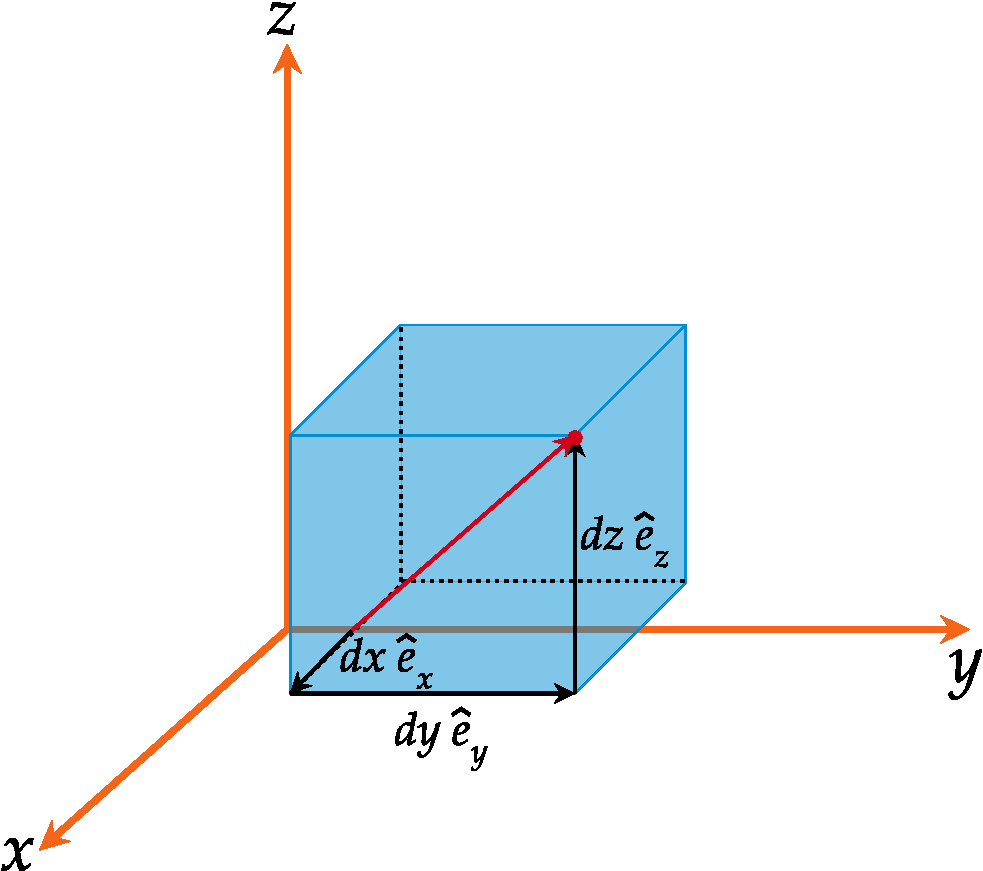
\includegraphics[scale=0.4]{cs-05-crop.pdf}
		\caption{line element}
		\label{line element}
	\end{minipage}
	\begin{minipage}{0.35\textwidth}
		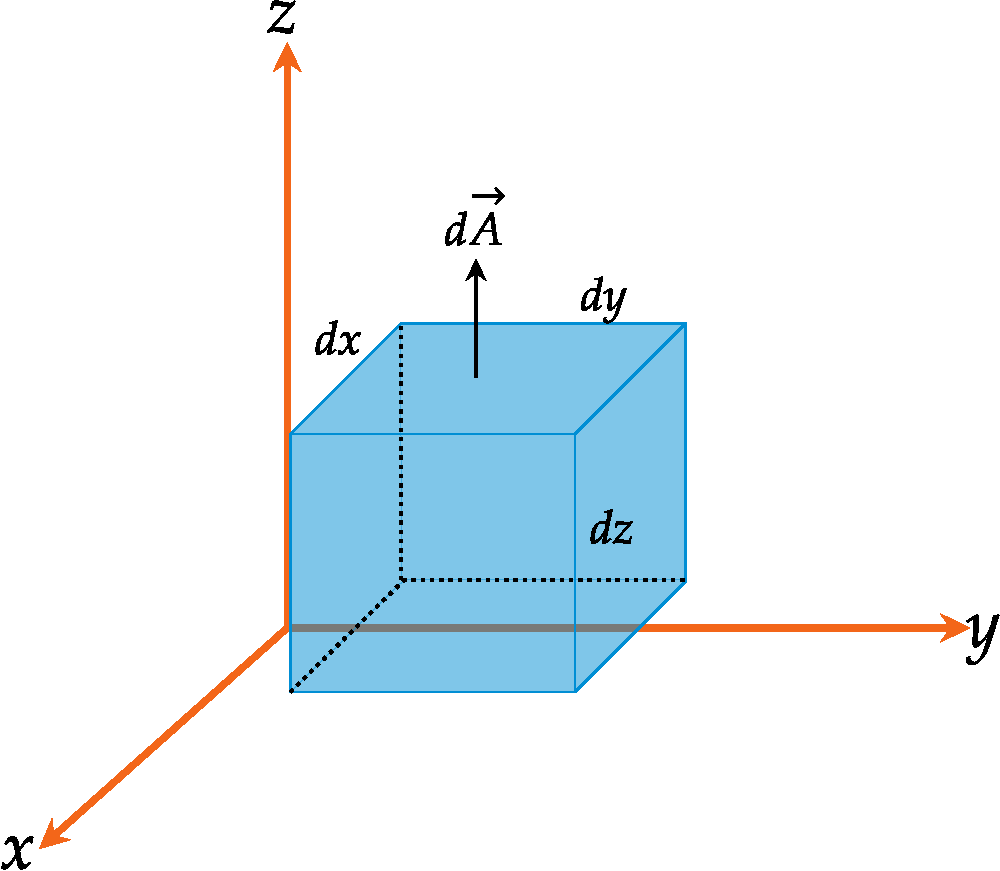
\includegraphics[scale=0.4]{cs-03-crop.pdf}
		\caption{Area element}
	\end{minipage}
	\begin{minipage}{0.30\textwidth}
		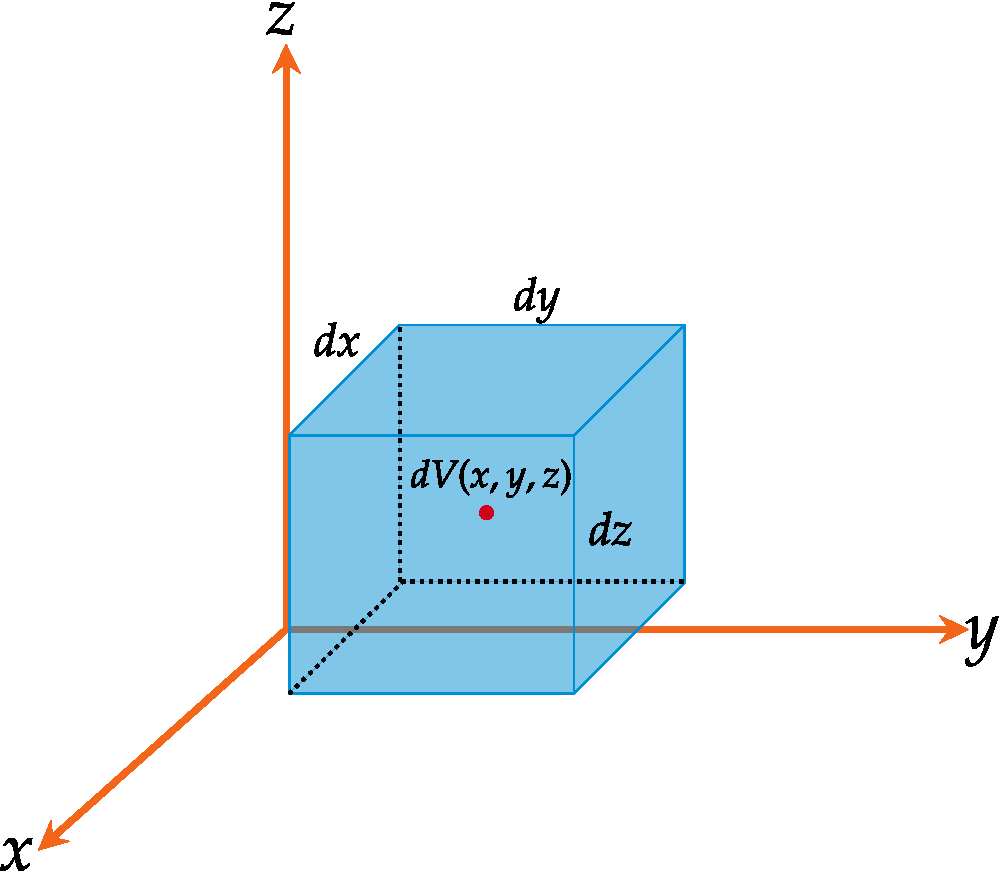
\includegraphics[scale=0.4]{cs-06-crop.pdf}
		\caption{Volume element}
	\end{minipage}
\end{figure}
\begin{itemize}
	\item{\textbf{Line element}}\\
	Consider a small infinitesimal displacement $dl$  between two points $p_{1}$ and $p_{2}$ as in the fig.\ref{line element} then it  is defined as, \begin{align*}
	d {\vec{l}}&=d x \hat{e_{x}}+d y \hat{e_{y}}+d z \hat{e_{z}}
	\end{align*}
	\item{\textbf{Area element}}\\ The infinitesimal area element in a cartesian coordinate system is defined as ,
	\begin{align*}
	d\vec{A}&=dx dy \hat{e_{z}}\qquad \text{Area element in the x-y plane.}\\
	\intertext{Similiarly, }\
	d\vec{A}&=dx dz \hat{e_{y}} \qquad \text{Area element in the x-z plane.}\\
	\text{And}\quad  d\vec{A}&=dy dz  \hat{e_{x}} \qquad \text{Area element in the y-z plane.}
	\end{align*}
	\item{\textbf{Volume element}}\\ The infinitesimal volume element in a cartesian coordinate system is defined as,
	\begin{equation*}
	d{V}=dx dy dz 
	\end{equation*}
	Remember that the infinitesimal volume element is a scalar quantity.	
	
	
\end{itemize}
\subsection{Kinematic Vectors in Cartesian Coordinate System}
\begin{itemize}
	\item \textbf{Velocity}
	\begin{align*}
	\intertext{We know that velocity is the rate of change of displacement. So, differentiating the displacement vector we get,}
	\text { Velocity }, \vec{v}&=\frac{d \vec{r}}{d t}\\
	\text{Velocity in cartesian coordinate system:} \\
	\vec{v}&=\frac{d \vec{r}}{d t}=\frac{d}{d t}(x \hat{e_{x}}+y \hat{e_{y}}+z \hat{e_{z}})\\&=\dot{x} \hat{e_{x}}+\dot{y} \hat{e_{y}}+\dot{z} \hat{e_{z}}\\
	\text{Where,} \ \dot{x}&=\frac{dx}{dt}\quad ;\quad \dot{y}=\frac{dy}{dt}\quad ;\quad\dot{z}=\frac{dz}{dt}
	\end{align*}
	
	\item \textbf{Acceleration}
	\begin{align*}
	\intertext{Acceleration is the rate of change of velocity. differentiating velocity vector with respect to time we get acceleration .}
	\text{Accelaration} ,\ \vec{a}&=\frac{d \vec{v}}{d t}\\
	\text{Accelaration in cartesian coordinate system:}\\ \vec{a}&=\frac{d \vec{v}}{d t}=\frac{d \dot{\vec{x}}}{d t}+\frac{d \dot{\vec{y}}}{d t}+\frac{d \dot{\vec{z}}}{d t}\\&=\ddot{x} \hat{e_{x}}+\ddot{y} \hat{e_{y}}+\ddot{z} \hat{e_{z}}
	\end{align*}
	
	
\end{itemize}

%.........................
\section{Polar Co-Ordinate System}
The polar coordinate system is just an another way of describing the locations of points in a plane. We need to use polar coordinates , where there is circular  symmetry in the form of a physical object, or some kind of circular or orbital (oscillatory) motion. A polar equation describes a relationship between $\rho$ and $\phi$ on a polar grid. One of the main  application of polar coordinates is in orbital motions of celestial objects.  Instead of giving x and y coordinates, we’ll describe the location of a point by,\\
\begin{minipage}{0.45\textwidth}
	\begin{itemize}
		\item {$\rho$= Distance  from origin}
		\item{$\phi$= Angle between the ray from the origin to the point and the horizontal
			axis.}
		\begin{align*}
		x&=\rho \cos \phi
		\quad;\quad y=\rho\sin \phi
		\intertext{ $\rho$ and $\phi$ varies as,}
		0 &\leq \rho \leq \infty\\ 0 &\leq \phi\leq 2 \pi
		\end{align*}
	\end{itemize}
\end{minipage}\hfill
\begin{minipage}{0.45\textwidth}
	\begin{figure}[H]
		\centering
		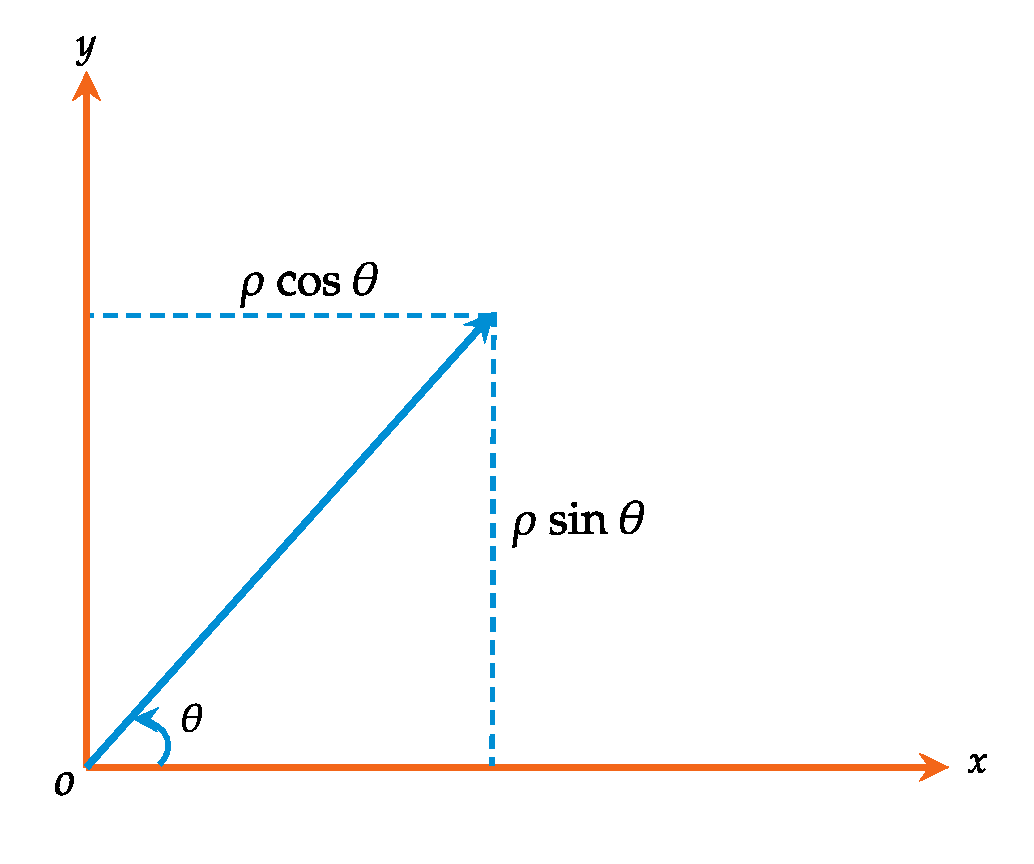
\includegraphics[width=6cm,height=5cm]{polar}
		\caption{ Polar Coordinate system}
		\label{ Polar Coordinate system}
	\end{figure}
\end{minipage}\\\\
In the plane polar coordinates the condition $\rho=\text{Constant}$ , provides circles, where as $\phi=\text{Constant }$ provides radial line.
Since we are dealing with free vectors, we can translate the polar reference frame for a given point $(\rho, \phi),$ to cartesian, by  a standard change of basis procedure.
\\So that the inverse relationships to convert rectangular coordinates to polar coordinates, we can  use,

\begin{align*}
x&= \rho \cos \phi\\
y&= \rho \sin \phi\\
\rho &=\sqrt{x^{2}+y^{2}} \\
\phi &=\tan ^{-1} \frac{y}{x}
\end{align*}

\subsection{Position Vector and Unit Vector}
\begin{align*}
\intertext{The position vector $\vec{r}$ in polar coordinate is given by :}
\vec{r}&=\rho\hat{{e_{\rho}}}\\
\intertext{In the polar coordinate system we have $\hat{e_{\rho}}$ in the increasing direction of $\rho$ and  $\hat{e_{\phi}}$ in the increasing direction of $\phi$. Since the direction of the unit vectors depend on the position of the point both $\hat{e_{\rho}}$ and $\hat{e_{\phi}}$ are a function of $\phi$,}
\intertext{The unit vectors are defined as ,}  \hat{e_{\rho}}&=\frac{\partial \vec{r} / \partial \rho}{|\partial \vec{r} / \partial \rho|}=\cos \phi \hat{e_{x}}+\sin \phi \hat{e_{y}}\\ \hat{e_{\phi}}&=\frac{\partial \vec{r} / \partial \phi}{|\partial \vec{r} / \partial \phi|}=-\sin \phi \hat{e_{x}}+\cos \phi \hat{e_{y}}
\intertext{In matrix notation,}
\left(\begin{array}{c}
\hat{e_{\rho}} \\
\hat{e_{\phi}}
\end{array}\right)&=\left(\begin{array}{cc}
\cos \phi & \sin \phi \\
-\sin \phi & \cos \phi
\end{array}\right)\left(\begin{array}{c}
\hat{e_{x}} \\
\hat{e_{y}}
\end{array}\right)\\\\
\hat{e_{\rho}} \times \hat{e_{\phi}}&=\hat{e_{z}}
\end{align*}
Since the unit vectors transforms this way components of any general vector $A$ should transform in the same way. And we have the transformation matrix,
\begin{align*}
\left(\begin{array}{c}
A_{\rho} \\
A_{\phi}
\end{array}\right)&=\left(\begin{array}{cc}
\cos \phi & \sin \phi \\
-\sin \phi & \cos \phi
\end{array}\right)\left(\begin{array}{c}
A_{x} \\
A_{y}
\end{array}\right) \\\intertext { And } \quad\left(\begin{array}{c}
A_{x} \\
A_{y}
\end{array}\right)&=\left(\begin{array}{cc}
\cos \phi & -\sin \phi \\
\sin \phi & \cos \phi
\end{array}\right)\left(\begin{array}{c}
A_{\rho} \\
A_{\phi}
\end{array}\right)
\end{align*}

\subsection{Line, Area and Volume Elements}
\begin{itemize}
	\item \textbf{Line element}
	\begin{align*}
	\vec{dl}=d \rho \hat{e_{\rho}}+\rho d \hat{e_{\phi}}
	\end{align*}
	\item \textbf{Area element} \begin{align*}
	d \vec{A}&=d \rho \hat{e_{\rho}} \times \rho d \phi \hat{e_{\phi}}\\&=\rho d \rho d \phi \hat{e_{z}}
	\end{align*}
\end{itemize}
	\begin{figure}[h]
	\begin{minipage}{0.45\textwidth}
		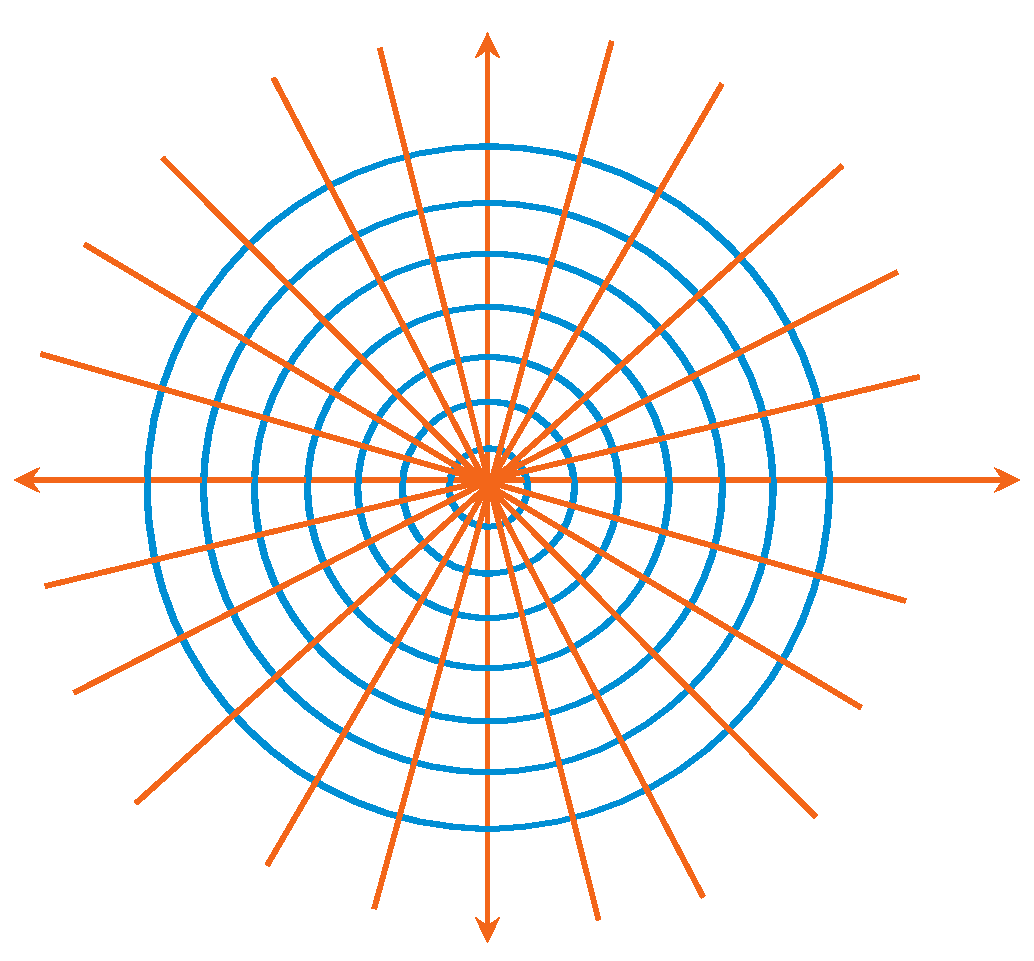
\includegraphics[width=6cm,height=5.5cm]{diagram-20211126(3)}
		\caption{Circular symmetry of Polar coordinate system}
		
	\end{minipage}\hfill
	\begin{minipage}{0.45\textwidth}
		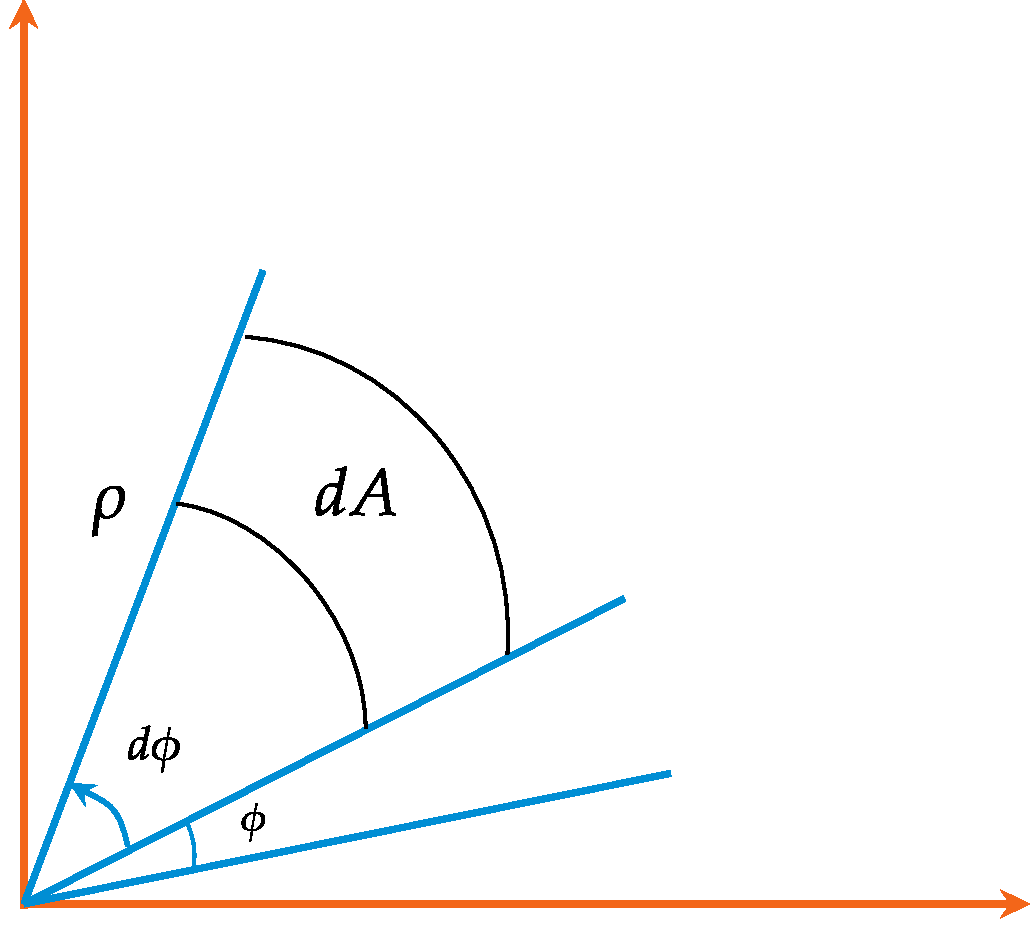
\includegraphics[width=6cm,height=5.5cm]{diagram-20211126(2)}
		\caption{Area element}
	\end{minipage}
\end{figure}
\subsection{Kinematic in Polar Coordinate System}
\begin{itemize}
	\item {\textbf{Velocity vector}}
	\begin{equation*}
	\text{Velocity }=\vec{v}=\frac{d \vec{r}}{d t}
	\end{equation*}
	But here the displacement vector is given by, $\vec{r}=\rho \hat{e_{\rho}}$
	\\\\Since the unit vectors  changes with time, they should have finite time derivatives:
	\begin{align*}
	\frac{d }{dt} e_{\rho}&=\dot{\hat{e_{\rho}}}\\&=\dot{\phi}(-\sin \phi \hat{e_{x}}+\cos \phi \hat{e_{y}})\\&=\dot{\phi} \hat{e_{\phi}}\\
	\text{And}\quad	\frac{d }{dt} e_{\rho}&=  \dot{\hat{e_{\phi}}}\\&=\dot{\phi}(-\cos \phi \hat{e_{x}}-\sin \phi \hat{e_{y}})\\&=-\dot{\phi} \hat{e_{\rho}}\\
	\intertext{Therefore the velocity is given by:}
	\vec{v}&=\frac{d \vec{\rho}}{d t}=\dot{\rho} \hat{e_{\rho}}+\rho \dot{\hat{e_{\rho}}}\\&=\dot{\rho} \hat{e_{\rho}}+\rho \dot{\phi} \hat{e_{\phi}}\\
	\text{Where,}\quad v_{\rho}&=\dot{\rho} \hat{e_{\rho}} \hspace{0.62cm} -\text{Radial velocity component.}\\
	v_{\phi}&=\rho \dot{\phi} \hat{e_{\phi}}\quad -\text{Tangential / Azimuthal velocity component.}
	\end{align*}
	
	\item{\textbf{Acceleration vector}}\\
	Differentiating again with respect to time, we obtain the acceleration
	\begin{align*}
	\boldsymbol{a}&=\dot{\boldsymbol{v}}=\ddot{\rho} \hat{e_{\rho}}+\dot{\rho} \dot\hat{e_{\rho}}+\dot{\rho} \dot{\phi} \hat{e_{\phi}}+\rho \ddot{\phi} \hat{e_{\phi}}+\dot{\rho} \dot{\boldsymbol{\phi}} \hat{\dot{\phi}}\\
	\boldsymbol{a}&=\left(\ddot{\rho}-\rho \dot{\phi}^{2}\right) \hat{e_{\rho}}+(\rho \ddot{\phi}+2 \dot{\rho} \dot{\phi}) \hat{e_{\phi}}\\
	a_{\rho}&=\left(\ddot{\rho}-\rho \dot{\phi}^{2}\right) \hspace{0.62cm}-\text{ Radial acceleration component.}\\
	a_{\phi}&=(\rho \ddot{\phi}+2 \dot{\rho} \dot{\phi})\quad -\text{ Azimuthal acceleration component.}\\
	|a|&=\sqrt{a_{\rho}^{2}+a_{\phi}^{2}}
	\end{align*}
	
\end{itemize}
%--------------------------------------------
The Cylindrical and spherical polar systems are the three-dimensional relatives of the two-dimensional polar coordinate system. Let us look into those systems.
\section{ Cylindrical Polar Co-Ordinate System}

\begin{wrapfigure}{r}{0.32\textwidth}
	\begin{center}
		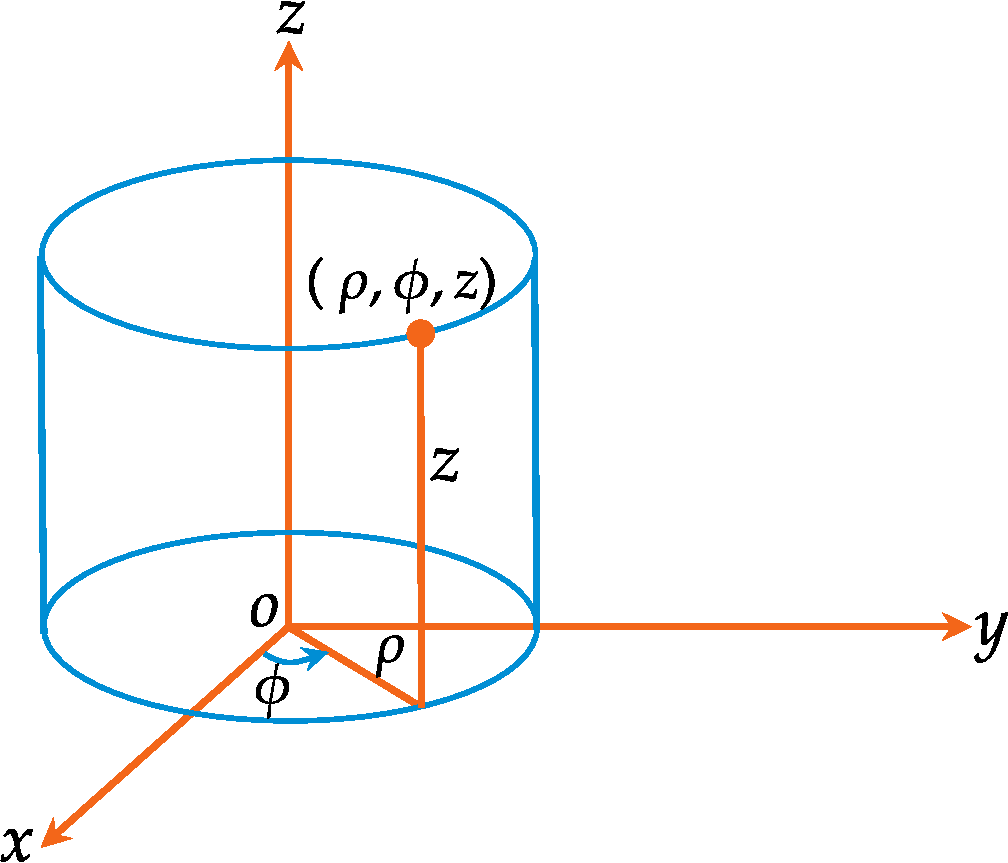
\includegraphics[width=6cm,height=5cm]{cylindrical 1}
	\end{center}
	\caption{Cylindrical Polar Coordinate system}
	\label{Cylindrical Polar Coordinate system}
\end{wrapfigure}
We make the use of Cylindrical polar coordinate system when there is a \textbf{cylindrical symmetry} in the form of a physical object.  Polar coordinates can be extended to three dimensions in a very straightforward manner. We simply add
the z coordinate, which is then treated in a cartesian like manner. Every point in space is determined by
the $\rho$ and $\theta$ coordinates of its projection in the xy plane, and its z coordinate.
\\ In the figure  \ref{Cylindrical Polar Coordinate system} ,$\rho$\ is the distance of the foot of the perpendicular drawn from the point to the $x-y(\rho, \theta)$\ plane.
Note that $\rho$ here is not the distance of the point $\mathrm{P}$ from the origin, as is the case in polar coordinate systems.\\The range of the coordinate varies as,\begin{align*}
0 &\leq \rho \leq \infty\\
0 &\leq \phi \leq 2 \pi\\
-\infty &\leq z \leq+\infty
\intertext{In terms of cartesian coordinates  }
x&=\rho \cos \phi \\
y&=\rho \sin \phi \\
z&=z
\end{align*}
We can change the basis of a 
vector in cylindrical coordinate system to cartesian. Any vector $\vec{A}$ can be expressed in terms of them in the usual way,
$$
\vec{A}=A_{\rho} \hat{e_{\rho}}+A_{\phi} \hat{\phi}+A_{z} \hat{z}
$$
In matrix form we can write,
$$
\begin{aligned}
&\left[\begin{array}{c}
A_{\rho} \\
A_{\phi} \\
A_{z}
\end{array}\right]=\left[\begin{array}{ccc}
\cos (\phi) & \sin (\phi) & 0 \\
-\sin (\phi) & \cos (\phi) & 0 \\
0 & 0 & 1
\end{array}\right]\left[\begin{array}{l}
A_{x} \\
A_{y} \\
A_{z}
\end{array}\right]
\end{aligned}
$$

\subsection{ Unit Vectors}
The unit vectors $\hat{e_{\rho}}, \hat{\phi}$ and $\hat{e_{z}},$ expressed in cartesian coordinates, are,
$$
\begin{array}{l}
\hat{e_{\rho}}=\cos \phi \hat{e_{x}}+\sin \phi \hat{e_{y}} \\
\hat{e_{\phi}}=-\sin \phi \hat{e_{x}}+\cos \phi \hat{e_{y}}\\
\hat{e_{z}}=\hat{e_{z}}
\end{array}
$$

\subsection{Line, Area and Volume Elements}
\begin{itemize}
	\item  \textbf{Line element} 
	$$
	\overrightarrow{d l}= d \rho \hat{e_{\rho}}+\rho d \phi \hat{\phi}+d \hat{e_{z}}
	$$
	
	\item \textbf{Area element }
	\\ Orthogonal surfaces in cylindrical coordinate system can be generated in three ways.\\\\ i.e., $\rho=$ constant,  $\phi=$ constant,
	$\mathrm{z}=$ constant.
	\begin{align*}
	\rho&= \text{constant : A circular cylinder} \Rightarrow d A=\rho d \phi d z\\
	\phi&=\text{constant : A semi infinite plane with its edge along $\mathrm{z}$ axis} \Rightarrow d A= \phi d\rho   d z \\
	\mathrm{z}&= \text{constant : An infinite plane as in the rectangular system.}\Rightarrow d A= zd\phi d\rho   
	\end{align*}
	
	
	
	\begin{figure}[h]
		\begin{minipage}{0.30\textwidth}
			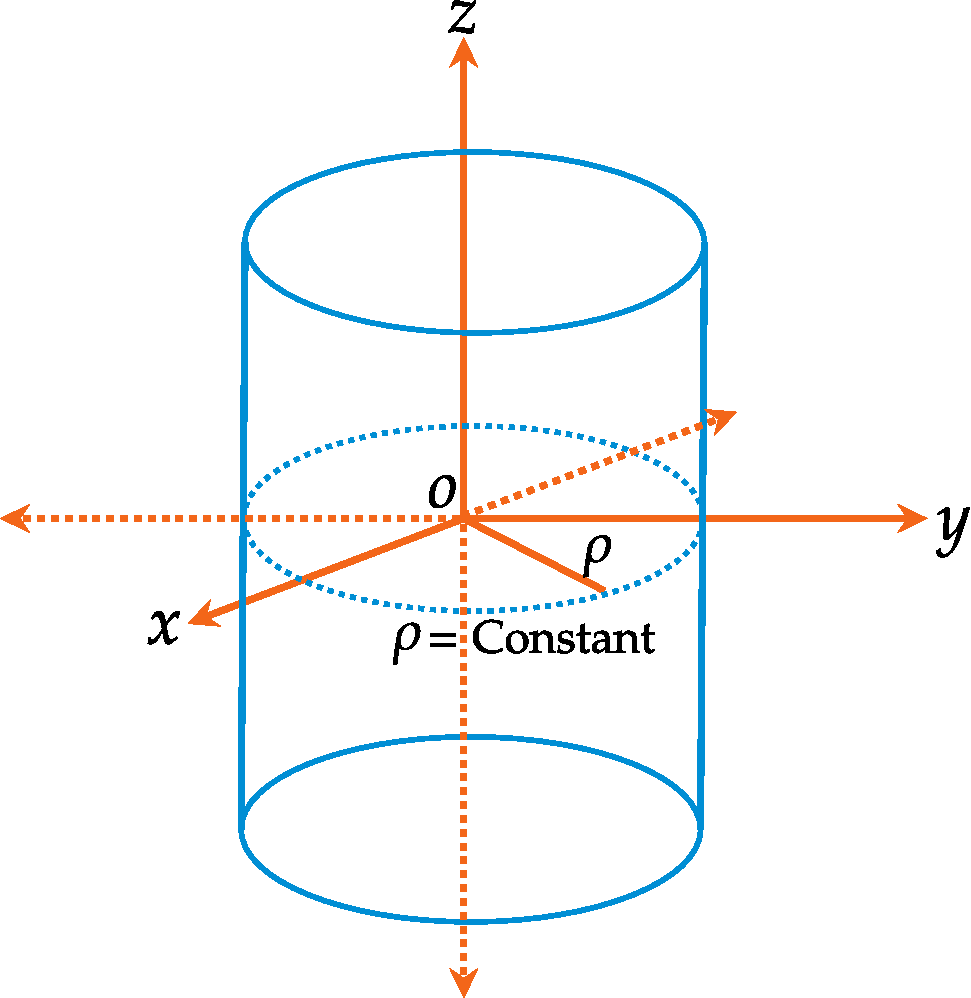
\includegraphics[width=6cm,height=6cm]{cylindrical 3}
			\caption{Constant $\rho$ surface}
			
		\end{minipage}\hspace{0.5cm}
		\begin{minipage}{0.35\textwidth}
			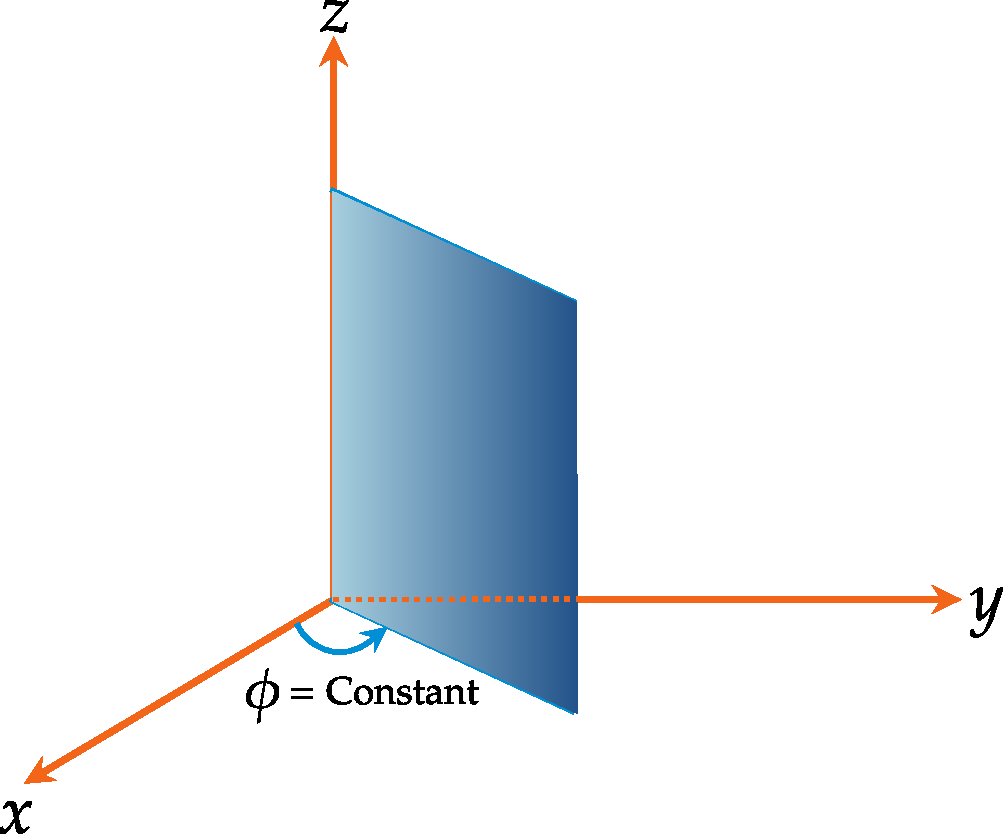
\includegraphics[width=6cm,height=6cm]{cylindrical 2}
			\caption{Constant $\phi$ surface}
		\end{minipage}
		\begin{minipage}{0.30\textwidth}
			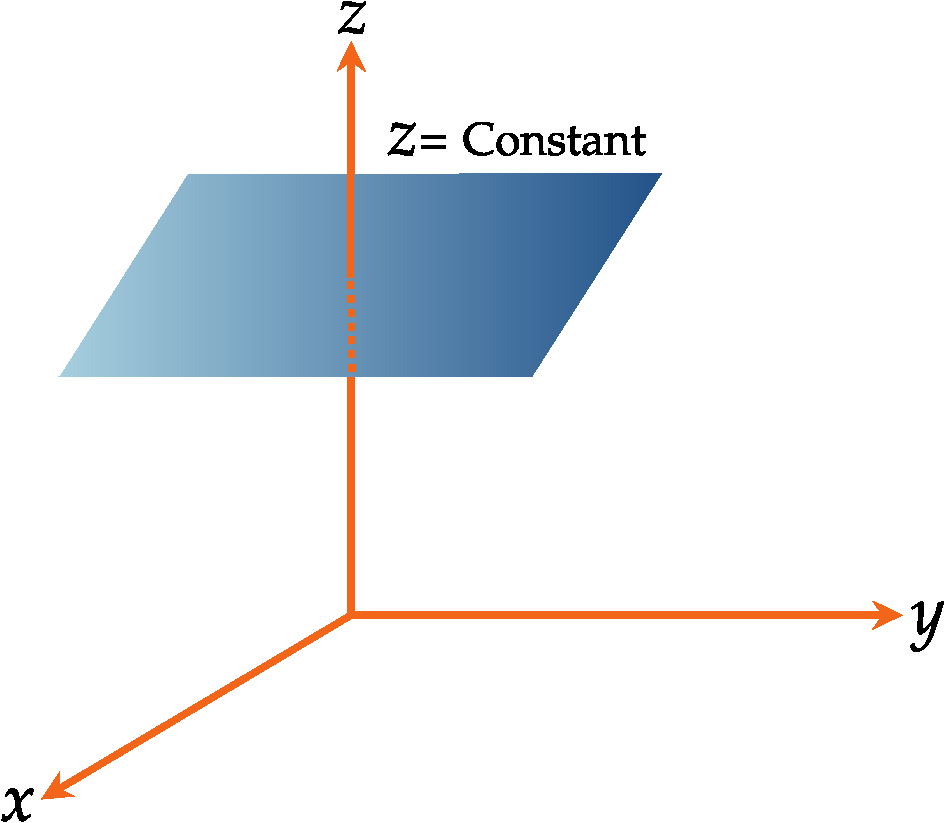
\includegraphics[width=6cm,height=6cm]{cylindrical 4}
			\caption{Constant $z$ surface}
		\end{minipage}
	\end{figure}
	\item   \textbf{Volume element}
	$$
	d V=\rho d \phi d \rho d z
	$$
	\end {itemize}
	
	\subsection{Kinematic Vectors in  Cylindrical Polar Coordinate System}
	\begin{itemize}
		\item \textbf{Velocity Vector}
		\begin{align*}
		\boldsymbol{v}&=\dot{\rho} \hat{e_{\rho}}+{\rho} \dot{\phi} \hat{\phi}+\dot{z} \boldsymbol{k}\\
		\text{Where,}\quad  v_{\rho}&=\dot{\rho}\quad;\quad v_{\phi}=r \dot{\phi}\quad;\quad v_{z}=\dot{z}\\ \text{And} \quad
		v&=\sqrt{v_{\rho}^{2}+v_{\phi}^{2}+v_{z}^{2}} \\\intertext{Where $ \dot{\rho}$  is radial velocity in $ \hat{e_{\rho}} $ direction and $ r \dot{\phi}$  is tangential velocity in $ \hat{\phi} $ direction}
		\end{align*}
		
		\item \textbf{Acceleration Vector}
		\begin{align*}
		\boldsymbol{a}&=\left(\ddot{\rho}-\rho \dot{\phi}^{2}\right) \hat{e_{\rho}}+(\rho \ddot{\phi}+2 \dot{\rho} \dot{\phi}) \hat{\phi}+\ddot{z} \boldsymbol{k}\\
		\text{Where}  \quad a_{\rho}&=\ddot{\rho}-\rho \dot{\phi}^{2}\quad;\quad a_{\phi}=\rho \ddot{\phi}+2 \dot{\rho} \dot{\phi}\quad;\quad a_{z}=\ddot{z}\\ \text{And}\quad a&=\sqrt{a_{\rho}^{2}+a_{\phi}^{2}+a_{z}^{2}}
		\end{align*}
		
		
		\end {itemize}
		
		%------------------------------------------------------
		\section{Spherical Polar Co-Ordinate System}
		
		We make  use of Spherical polar coordinate system when there is a \textbf{Spherical symmetry} in the form of a physical object. 
		In spherical polar coordinates, we utilize two angles and a distance to specify the position of a particle. Every point in space is determined by
		the $r$ , $\theta$  and $\phi $ coordinates.
		The range of coordinates varies as, \\
		\begin{minipage}{0.45\textwidth}
			\begin{align*}
			0 &\leq r \leq \infty\\
			0 &\leq \theta \leq \pi\\
			0&\leq \phi \leq 2\pi
			\end{align*}
			If you are given spherical coordinates $(r, \theta, \phi)$ of a point in the plane.The Cartesian coordinates $(x, y, z)$ can be determined from the coordinate transformations.
			
			\begin{align*}
			x&=r \sin \theta \cos \phi \\
			y&=r \sin \theta \sin \phi \\
			z&=r \cos \theta
			\end{align*}
		\end{minipage}
	\begin{minipage}{0.45\textwidth}
	\begin{figure}[H]
		\centering
	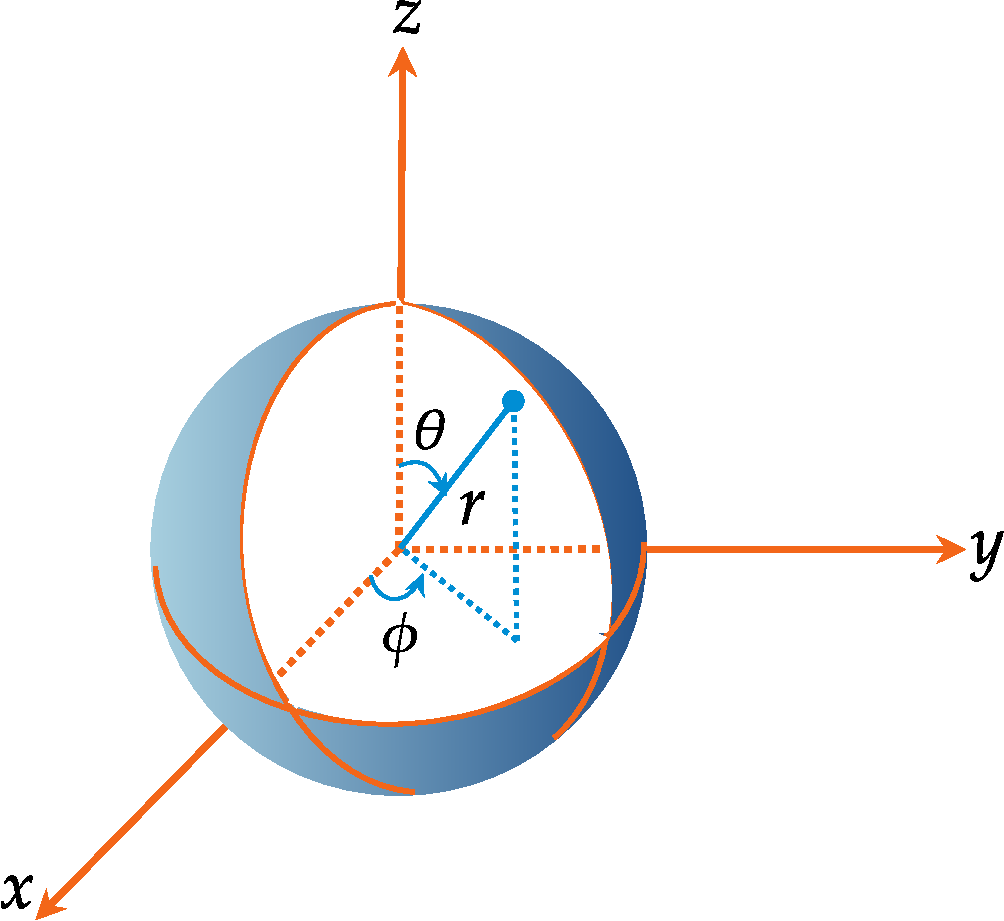
\includegraphics[width=7cm,height=6.5cm]{spherical 1}
		\caption{Spherical Polar Coordinate system}
		\label{Spherical Polar Coordinate system}
	\end{figure}
	\end{minipage}
		
	
		\subsection{Unit Vectors}
		Curresponding to radial distance(r), polar distance ($\theta$) and azimuthal angle ($\phi$) We have three orthogonal unit vectors in SPC and they constitute an orthonormal basis $\left\lbrace \hat{e_{r}},\hat{e_{\theta}},\hat{e_{\phi}} \right\rbrace $. The unit vectors also are related by the coordinate transformations
		$$
		\begin{array}{l}
		\hat{e_{r}}=\sin \theta \cos \phi \hat{e_{x}}+\sin \theta \sin \phi \hat{e_{y}}+\cos \theta \hat{e_{z}} \\
		\hat{e_{\theta}}=\cos \theta \cos \phi \hat{e_{x}}+\cos \theta \sin \phi \hat{e_{y}}-\sin \theta \hat{e_{z}} \\
		\hat{e_{\phi}}=-\sin \phi \hat{e_{x}}+\cos \phi \hat{e_{y}}
		\end{array}
		$$
		 In matrix representation,
		$$\left[\begin{array}{c}
			\hat{e_{r}} \\
			\hat{e_{\theta}} \\
			\hat{e_{\phi}}
		\end{array}\right]=\left[\begin{array}{ccc}
			\sin \theta \cos \phi & \sin \theta \sin \phi & \cos \theta \\
			\cos \theta \cos \phi & \cos \theta \sin \phi & -\sin \theta \\
			-\sin \phi & \cos \phi & 0
		\end{array}\right]\left[\begin{array}{c}
			\hat{e_{x}} \\
			\hat{e_{y}} \\
			\hat{e_{z}}
		\end{array}\right]$$
		The inverse transformation will be
			$$\left[\begin{array}{c}
			\hat{e_{x}} \\
			\hat{e_{y}} \\
			\hat{e_{z}}
		\end{array}\right]=\left[\begin{array}{ccc}
		\sin \theta \cos \phi & \cos \theta \cos \phi & -\sin \phi \\
		\sin \theta \sin \phi & \cos \theta \sin \phi & \cos \phi \\
		\cos \theta & -\sin \theta & 0
		\end{array}\right]\left[\begin{array}{c}
		\hat{e_{r}} \\
		\hat{e_{\theta}} \\
		\hat{e_{\phi}}
		\end{array}\right]$$
			Then any vector $\vec{A}$ can be expressed in terms of them in the usual way:
		\begin{align*}
		\vec{A}&=A_{r} \hat{e_{r}}+A_{\theta} \hat{e_{\theta}}+A _{\phi} \hat{e_{\phi}}\\
		A_{r}&=A_{x} \sin \theta \cos \phi+A_{y} \sin \theta \sin \phi+A_{z} \cos \theta\\
		A_{\theta}&=A_{x} \cos \theta \cos \phi+A_{y} \cos \theta \sin \phi-A_{z} \sin \theta\\
		A_{\phi}&=-A_{x} \sin \phi+A_{y} \cos \phi
		\intertext{	In matrix form we can write}
		\left[\begin{array}{c}
		A_{r} \\
		A_{\theta} \\
		A_{\phi}
		\end{array}\right]&=\left[\begin{array}{ccc}
		\sin \theta \cos \phi & \sin \theta \sin \phi & \cos \theta \\
		\cos \theta \cos \phi & \cos \theta \sin \phi & -\sin \theta \\
		-\sin \phi & \cos \phi & 0
		\end{array}\right]\left[\begin{array}{c}
		A_{x} \\
		A_{y} \\
		A_{z}
		\end{array}\right]
		\end{align*}
		\subsection{Line, Area ,Volume Elements}
		\begin{itemize}
			\item\textbf{ Line element}$$d \vec{{l}}=d r \hat{e_{r}}+r d \theta \hat{e_{\theta}}+r \sin \theta d \phi \hat{e_{\phi}}$$
			\item \textbf{Area element}\\
			\\ Orthogonal surfaces in Spherical polar coordinate system can be generated in three ways \\ i.e., $r=$ constant $\phi=$ constant and 
			$\mathrm{z}=$ constant.
			\begin{align*}
			r&= \text{constant : A sphere.}\Rightarrow d A_{r}=r^{2} \sin \theta d \theta d \phi  \\
			\theta&=\text{constant : A cone.} \Rightarrow d A_{\theta}=r \sin \theta d r d \phi \\
			\phi&= \text{constant : An semi infinite plane as in the rectangular system.} \Rightarrow d A_{\phi}=r d r d \theta 
			\end{align*}
			
			\begin{figure}[h]
				\begin{minipage}{0.30\textwidth}
					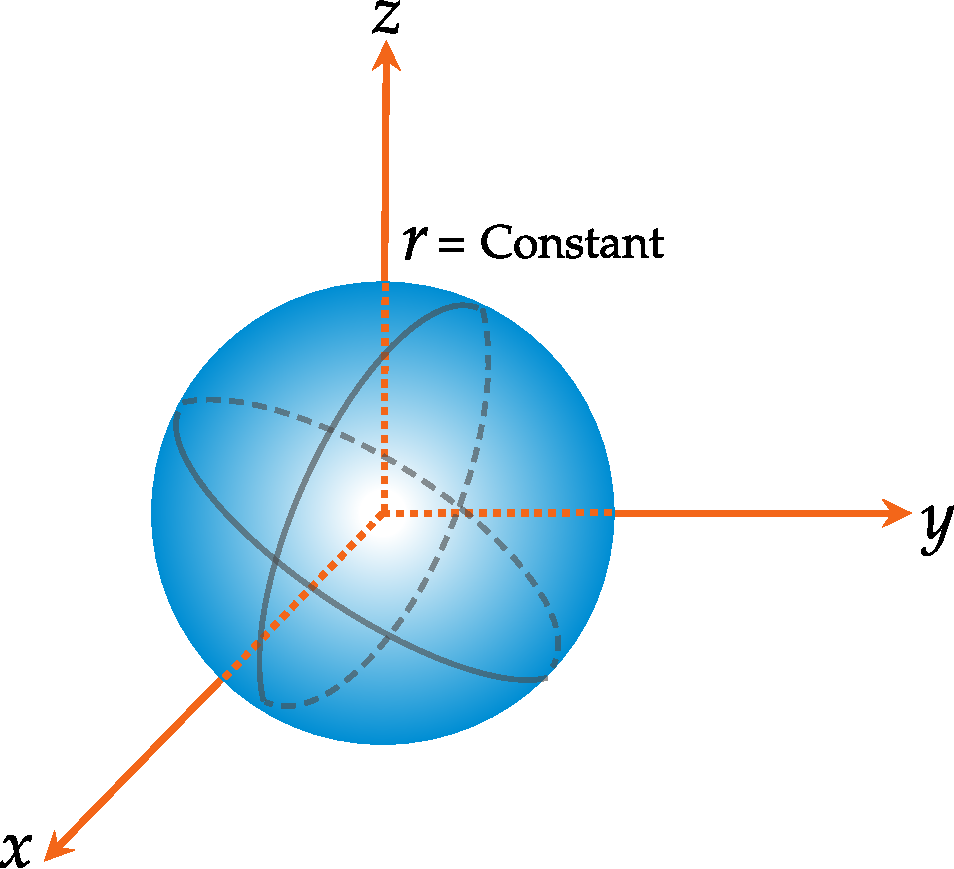
\includegraphics[width=6.5cm,height=6cm]{spherical 2}
					\caption{Constant $r$ surface}
				\end{minipage}\hspace{0.5cm}
				\begin{minipage}{0.35\textwidth}
					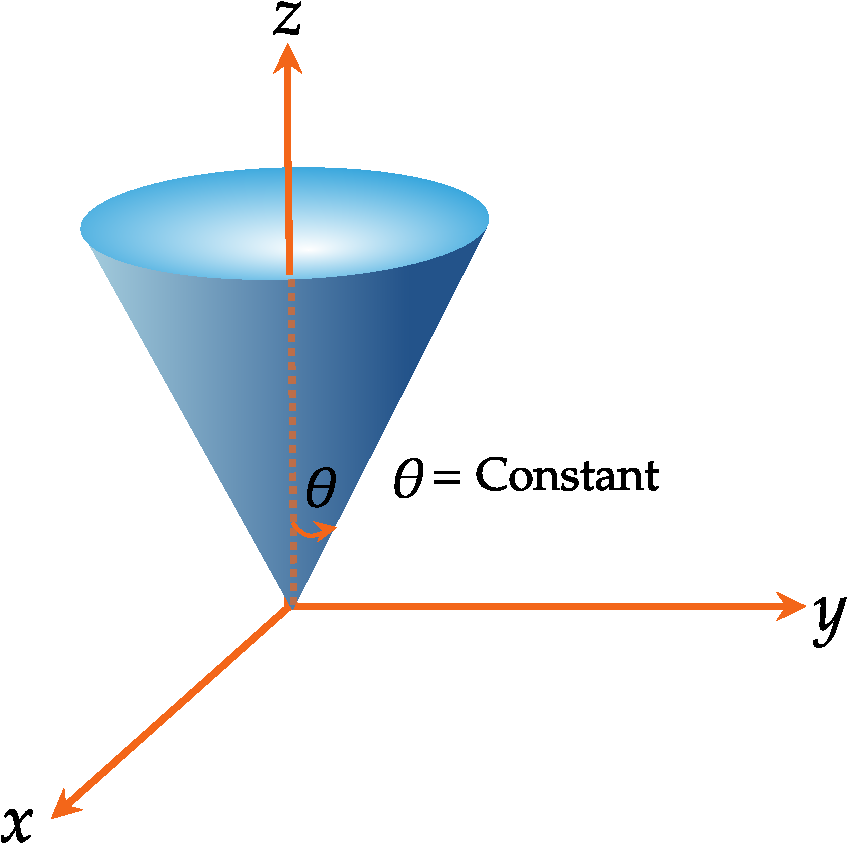
\includegraphics[width=6cm,height=6cm]{spherical 5}
					\caption{Constant $\theta$ surface}
				\end{minipage}
				\begin{minipage}{0.30\textwidth}
					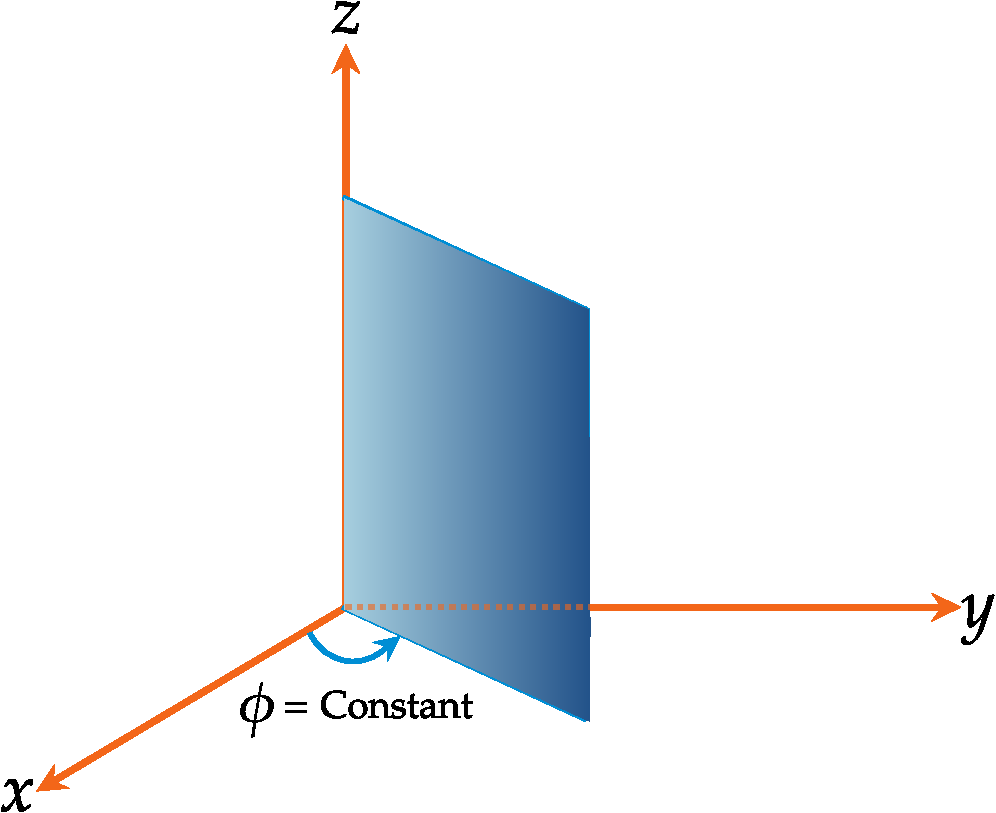
\includegraphics[width=6.5cm,height=6cm]{spherical 4}
					\caption{Constant $\phi$ surface}
				\end{minipage}
			\end{figure}
			
			\item \textbf{Volume elment}
			$$
			d V=r^{2}d r \sin \theta d \theta d \phi 
			$$
		\end{itemize}
		
		\subsection{Kinematic Vectors in Spherical Polar Coordinate System}
		\begin{itemize}
			\item	\textbf{Velocity Vector}\begin{align*}
			\vec{v}&=\dot{\vec{r}}\\&=\dot{\hat{e_{r}}} r+\hat{e_{r}} \dot{r} \\
			\vec{v}&=\hat{e_{r}} \dot{r}+\hat{e_{\theta}} r \dot{\theta}+\hat{e_{\phi}} r \dot{\phi} \sin \theta
			\end{align*}
			\item \textbf{Acceleration Vector}
			\begin{align*}
			\vec{a}=&\hat{e_{r}}\left(\ddot{r}-r \dot{\theta}^{2}-r \dot{\phi}^{2} \sin ^{2} \theta\right)+\hat{e_{\theta}}\left(r \ddot{\theta}+2 \dot{r} \dot{\theta}-r \dot{\phi}^{2} \sin \theta \cos \theta\right)\\&+\hat{e_{\phi}}(r \ddot{\phi} \sin \theta+2 r \dot{\theta} \dot{\phi} \cos \theta+{2 \dot{r} \dot{\phi} \sin \theta})\\
			\intertext{Where,}
			a_{r}&=\left(\ddot{r}-r \dot{\theta}^{2}-r \dot{\phi}^{2} \sin ^{2} \theta\right)\\
			a_{\theta}&=\left(r \ddot{\theta}+2 \dot{r} \dot{\theta}-r \dot{\phi}^{2} \sin \theta \cos \theta\right)\\
			a_{\phi}&=(r \ddot{\phi} \sin \theta+2 r \dot{\theta} \dot{\phi} \cos \theta+2 \dot{r} \dot{\phi} \sin \theta)
			\end{align*} 
			
			\end {itemize}
			
			%----------------------------------------------
			\begin{table}[H]
				\centering
				\renewcommand*{\arraystretch}{2}
				\arrayrulecolor{ocre}
				
				\begin{tabular}{|p{3cm}|p{3.5cm}|p{2.5cm}|p{3.5cm}|}
					\hline
					\multicolumn{4}{|c|}{\textbf{Co-ordinate systems}}\\\hline
					\textbf{System}&\textbf{Symmetry}&\textbf{Co-ordinates}
					&\textbf{Length elements}\\\hline
					Cartesian &Rectangular &$x,y,z$&$dx,dy,dz$\\\hline 
					Polar&Circular symmetry &$r ,\theta $&$dr ,r d\theta $ \\\hline
					Cylindrical polar&Cylindrical symmetry &$r ,\theta,z $&$dr ,r d\theta, dz $ \\\hline
					Spherical polar&Spherical symmetry &$r ,\theta ,\phi$&$dr ,r d\theta, r \sin \theta d\phi $\\\hline
					
				\end{tabular}
				\caption{Basic summary of Coordinate system.}
			\end{table}
			
